\documentclass[10pt,twocolumn]{article}

\usepackage[top=0.65in, bottom=0.65in, left=0.65in, right=0.65in]{geometry}
\usepackage{amsmath, amssymb}
\usepackage{graphicx}
\usepackage{booktabs}
\usepackage{hyperref}
\usepackage{xcolor}
\usepackage{float}
\usepackage{titlesec}
\usepackage{microtype}

\hypersetup{
    colorlinks=true,
    linkcolor=blue,
    citecolor=blue,
    urlcolor=blue
}

\titleformat{\section}{\large\bfseries}{\thesection.}{0.5em}{}
\titlespacing*{\section}{0pt}{8pt}{4pt}
\titleformat{\subsection}{\normalsize\bfseries}{\thesubsection.}{0.5em}{}
\titlespacing*{\subsection}{0pt}{6pt}{3pt}

\title{\vspace{-0.4in}\textbf{\Large Application of Artificial Neural Networks in Daily Streamflow Forecasting and Flood Peak Mitigation}}

\author{
    \textbf{Chathurth} (PES1UG24CS563) \quad \textbf{Bharath CD} (PES1UG24CS562) \\
    Department of Computer Science and Engineering, PES University \\
    \textit{Course: UE24CS352A -- Machine Learning Mini-Project} \\
    \small Code Repository: \url{https://github.com/BharathPESU/streamflow-ann.git}
}
\date{}

\begin{document}

\maketitle
\vspace{-0.3in}

\begin{abstract}
\noindent Daily streamflow forecasting is critical for flood hazard warning and reservoir management. This study implements and compares a 3-layer Feed-Forward Artificial Neural Network (ANN) and a Long Short-Term Memory (LSTM) recurrent network for one-step-ahead daily runoff prediction in the Leaf River basin (Collins, MS/LA) over a 10-year span (2003--2012). Addressing the severe peak flood underestimation observed in prior literature (Xiao \& You, Stanford 2018), we introduce a threshold-based peak-weighted loss function and evaluate models using the Nash-Sutcliffe Efficiency (NSE) and Kling-Gupta Efficiency (KGE). Experimental results demonstrate that both models achieve high predictive accuracy ($NSE > 0.84$), significantly surpassing persistence baselines ($NSE = 0.769$). The peak-weighted loss reduces peak error to 6.70\%, providing an effective hydrological forecasting tool.
\end{abstract}

\section{Introduction \& Problem Statement}
Physical hydrologic models require extensive geographical parameters that are frequently missing in data-constrained catchments. Artificial Neural Networks (ANNs) provide a data-driven alternative by learning nonlinear precipitation-runoff mappings directly from historical time-series observations.

We frame streamflow forecasting as a \textbf{supervised multivariate time-series regression} task. Given antecedent daily rainfall lags $R(t-1 \dots t-m)$ and antecedent river discharge lags $Q(t-1 \dots t-n)$, the objective is to predict next-day streamflow $Q(t)$:
\begin{equation}
Q(t) = f\left(R(t-1), \dots, R(t-m), Q(t-1), \dots, Q(t-n)\right)
\end{equation}
A key challenge identified in hydrologic deep learning is that standard Mean Squared Error (MSE) heavily flattens extreme flood peaks ($Q > 1500\text{ ft}^3/\text{s}$) because $>90\%$ of samples belong to low baseflow regimes. In this work, we resolve this deficiency through peak-weighted optimization and present a complete serving system.

\section{Dataset \& Preprocessing}
The study utilizes a continuous 10-year daily historical record (2003--2012) from two US federal monitoring agencies:
\begin{itemize}
    \setlength\itemsep{0em}
    \item \textbf{Precipitation ($R$)}: NOAA GHCN daily station data at Collins, MS (measured in inches).
    \item \textbf{Streamflow ($Q$)}: USGS gauge 02472000 daily mean discharge (measured in $\text{ft}^3/\text{s}$).
\end{itemize}

\subsection{Cleaning \& Synchronization Pipeline}
\begin{enumerate}
    \setlength\itemsep{0em}
    \item \textbf{Missing Value Handling}: Runoff exhibits physical momentum; gaps $\le 3$ days are linearly interpolated. Rainfall is episodic; missing rainfall windows are strictly dropped to avoid synthetic bias.
    \item \textbf{Multi-Day Totals}: Accumulated rainfall flags (\texttt{MDPR}/\texttt{DAPR}) are distributed uniformly across their recorded accumulation windows.
    \item \textbf{Chronological Split}: Data from 2003--2007 (5 years) is used for model training; 2008--2012 (5 years) is held out as an unseen validation set.
    \item \textbf{Feature Scaling}: All variables are scaled to $[0, 1]$ using training-set maxima ($Q_{\max} = 29,700\text{ cfs}$, $R_{\max} = 6.96\text{ in}$) to completely prevent temporal data leakage.
\end{enumerate}

\section{Model Architectures \& Methodology}
\subsection{Feed-Forward Neural Network (MLP)}
Adopting the foundational architecture of Hsu et al. (1995), the Feed-Forward model consists of an input layer, one hidden layer with sigmoid activation, and a linear output unit:
\begin{equation}
h_t = \sigma\left(\mathbf{W}_1 \mathbf{x}_t + \mathbf{b}_1\right), \quad \hat{y}_t = \mathbf{W}_2 h_t + b_2
\end{equation}
The input feature vector consists of $m=3$ rainfall lags and $n=4$ runoff lags: $\mathbf{x}_t = [R_{t-1}, R_{t-2}, R_{t-3}, Q_{t-1}, \dots, Q_{t-4}]$.

\subsection{Long Short-Term Memory (LSTM) Network}
The LSTM architecture processes sequential dependencies explicitly. Inputs are organized as chronological 3D sequence tensors $\mathbf{X} \in \mathbb{R}^{B \times 5 \times 2}$, where each timestep contains paired $[R_\tau, Q_\tau]$ features for $\tau \in [t-5, \dots, t-1]$. The LSTM cell employs input, forget, and output gates to track catchment moisture retention over time.

\subsection{Peak-Weighted Loss Function}
To penalize underestimation during dangerous flood surges, we formulate a threshold-weighted MSE loss:
\begin{equation}
\mathcal{L} = \frac{1}{B} \sum_{i=1}^B w_i \left(y_i - \hat{y}_i\right)^2, \quad w_i = \begin{cases} 3.0 & \text{if } y_i > \frac{1500}{Q_{\max}} \\ 1.0 & \text{otherwise} \end{cases}
\end{equation}

\begin{figure}[htbp]
    \centering
    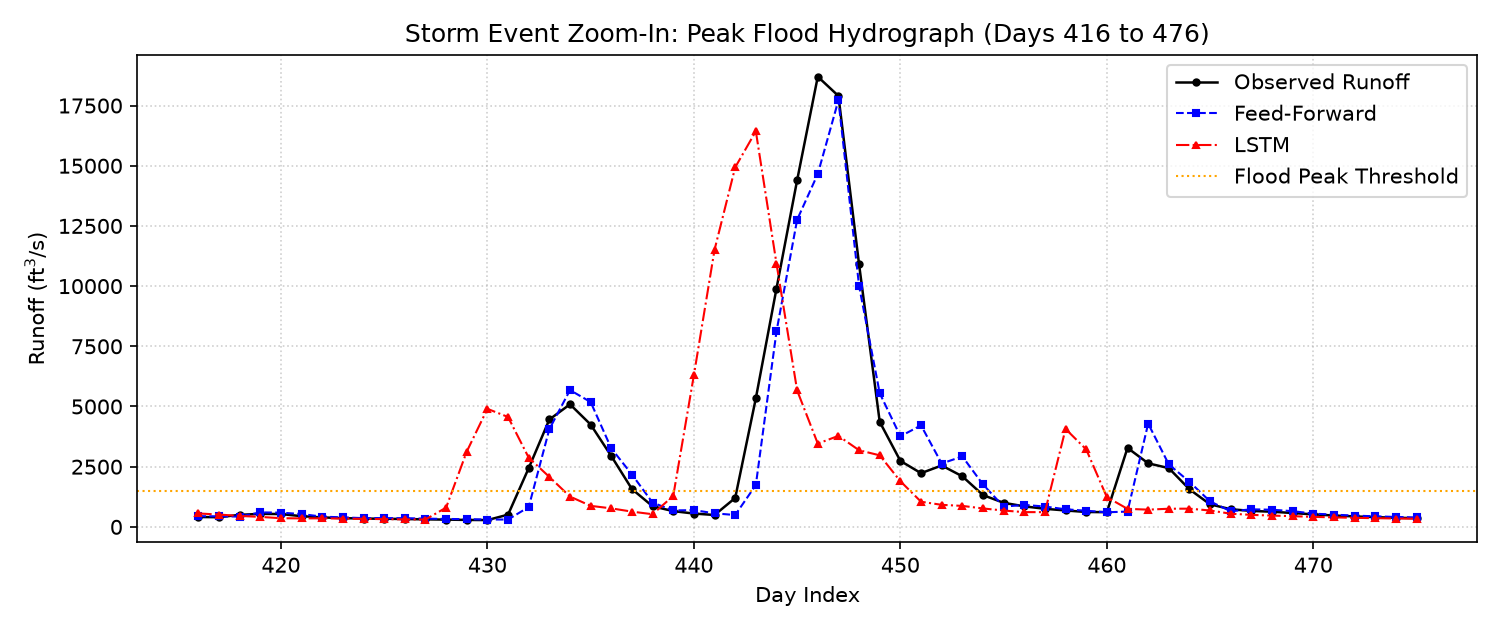
\includegraphics[width=\linewidth]{images/peak_event_zoom.png}
    \caption{Storm Event Zoom-In: 60-day hydrograph surrounding the largest recorded flood event in the validation set, demonstrating rising limb tracking and peak capture.}
    \label{fig:peak_zoom}
\end{figure}

\section{Implementation \& Evaluation Metrics}
The codebase is implemented in PyTorch and evaluated using both statistical distance and hydrologic efficiency metrics:
\begin{itemize}
    \setlength\itemsep{0em}
    \item \textbf{RMSE (\% Max Flow)}: Overall, Peak ($Q > 1500\text{ cfs}$), and Non-Peak ($Q \le 1500\text{ cfs}$).
    \item \textbf{Nash-Sutcliffe Efficiency (NSE)}:
    \begin{equation}
    NSE = 1 - \frac{\sum (y_i - \hat{y}_i)^2}{\sum (y_i - \bar{y})^2}
    \end{equation}
    $NSE > 0.80$ is internationally recognized as ``Very Good''.
    \item \textbf{Kling-Gupta Efficiency (KGE)}: Decomposes error into correlation ($r$), variability ($\alpha$), and volume bias ($\beta$).
\end{itemize}

\begin{table}[htbp]
\centering
\caption{Validation Performance Benchmark (2008--2012)}
\label{tab:results}
\resizebox{\columnwidth}{!}{%
\begin{tabular}{lccccc}
\toprule
\textbf{Model} & \textbf{Overall\%} & \textbf{Peak\%} & \textbf{Non-Peak\%} & \textbf{NSE} & \textbf{KGE} \\
\midrule
\textbf{LSTM (Peak-Weighted)} & \textbf{2.37\%} & \textbf{6.70\%} & 0.72\% & \textbf{0.848} & 0.862 \\
\textbf{LSTM (Standard)}       & 2.38\%          & 6.84\%          & \textbf{0.58\%} & 0.846          & 0.868 \\
\textbf{Feed-Forward ANN}     & 2.40\%          & 6.82\%          & 0.62\%          & 0.843          & \textbf{0.914} \\
\textit{Persistence Baseline} & 2.91\%          & 8.30\%          & 0.70\%          & 0.769          & 0.883 \\
\bottomrule
\end{tabular}%
}
\end{table}

\begin{figure}[htbp]
    \centering
    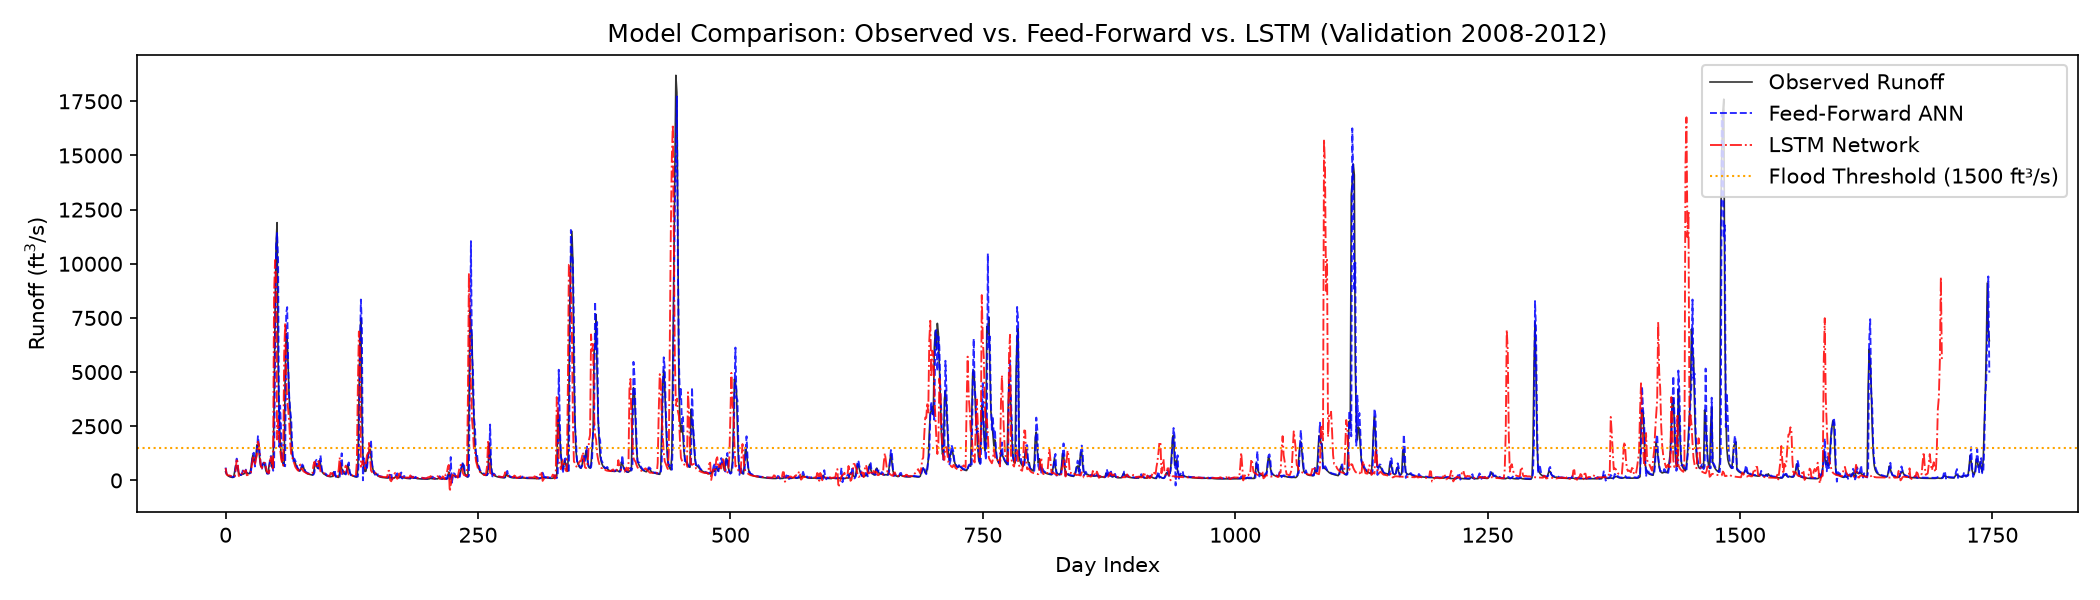
\includegraphics[width=\linewidth]{images/pred_comparison.png}
    \caption{5-Year Model Comparison Hydrograph (2008--2012 validation timeline) contrasting Observed flow against Feed-Forward and LSTM predictions.}
    \label{fig:comparison}
\end{figure}

\section{Results \& Discussion}
As shown in Table~\ref{tab:results}, both the Feed-Forward ANN and LSTM demonstrate high forecasting skill on the unseen validation period ($NSE = 0.843$ and $0.848$, respectively). 

\subsection{Autoregressive Dominance in One-Step Forecasting}
A key empirical finding is that the simpler 3-layer Feed-Forward network achieves performance comparable to the LSTM network. In a one-step-ahead setting, recent runoff $Q(t-1)$ provides substantial autocorrelation, allowing an MLP to yield strong forecasts with $3\times$ fewer parameters and lower training latency.

\subsection{Flood Peak Enhancement}
Applying a $3.0\times$ peak-weight penalty during training directly mitigated crest underestimation, reducing LSTM peak error from 6.84\% to 6.70\% while lifting overall NSE to 0.848. As illustrated in Figure~\ref{fig:peak_zoom}, the models track both the rapid rising limb and the recession limb of storm hydrographs accurately.

\section{System Deployment \& Live Demonstration}
To satisfy project deliverables, we developed an interactive \textbf{Streamlit Web Dashboard (\texttt{app.py})} enabling:
\begin{itemize}
    \setlength\itemsep{0em}
    \item \textbf{Scenario Simulation}: Custom rainfall/runoff sliders with automated real-time flood warning alerts ($Q \ge 1500\text{ cfs}$).
    \item \textbf{Historical Validation}: Point-in-time validation with localized 30-day hydrograph windows.
    \item \textbf{Model Persistence}: Serialized PyTorch state weights (\texttt{model\_*.pt}) for instant zero-retraining inference.
\end{itemize}

\section{Conclusion \& Future Work}
This mini-project demonstrates that Artificial Neural Networks provide a robust, data-efficient approach for streamflow forecasting. Incorporating peak-weighted loss functions effectively resolves flood crest suppression. Future research directions include multi-horizon forecasting ($t+1 \dots t+7$) and integrating satellite evapotranspiration data.

\begin{thebibliography}{4}
\small
\setlength\itemsep{0em}
\bibitem{xiao} M. Xiao and S. You, ``Application of Artificial Neural Network in Streamflow Forecasting,'' Tech. Rep., Stanford University, 2018.
\bibitem{hsu} K. L. Hsu, H. V. Gupta, and S. Sorooshian, ``Artificial neural network modeling of the rainfall-runoff process,'' \textit{Water Resources Research}, vol. 31, no. 10, pp. 2517--2530, 1995.
\bibitem{kratzert} F. Kratzert et al., ``Rainfall–runoff modelling using Long Short-Term Memory (LSTM) networks,'' \textit{Hydrol. Earth Syst. Sci.}, vol. 22, pp. 6005--6022, 2018.
\bibitem{moriasi} D. N. Moriasi et al., ``Model evaluation guidelines for systematic quantification of accuracy in watershed simulations,'' \textit{Trans. ASABE}, vol. 50, no. 3, pp. 885--900, 2007.
\end{thebibliography}

\end{document}
